\id{ҒТАМР 20.15.13}

{\bfseries МАШИНАЛЫҚ ОҚЫТУ ӘДІСТЕРІН ҚОЛДАНУ АРҚЫЛЫ СҮТ БЕЗДЕРІНІҢ
АУРУЛАРЫН ТИІМДІ ДИАГНОСТИКАЛАУ}

{\bfseries А.Р. Оразаева, Д.А. Тусупов\textsuperscript{\envelope }}

Л.Н. Гумилев атындағы Еуразия ұлттық университеті, Астана, Қазақстан

\raggedright {\bfseries \textsuperscript{\envelope }}Корреспондент-автор: \href{mailto:oaris.83@gmail.com}{tussupov@mail.ru}

Бұл мақала заманауи машиналық оқыту технологияларын, атап айтқанда, You
Only Look Once (YOLOv8) және Faster Region-based Convolutional Neural
Network (R-CNN) пайдалана отырып, сүт бездерінің патологиясын тиімді
анықтау әдістерін зерттеуге және дамытуға бағытталған. Мақалада сүт безі
ауруларын диагностикалаудың қолданыстағы тәсілдеріне талдау жасалып,
олардың тиімділігі бағаланады. YOLOv8 және Faster R-CNN архитектуралары
маммографиялық кескіндердегі патологияларды анықтау үлгілерін жасау үшін
қолданылады. Зерттеу әртүрлі ауырлық дәрежесін және аурудың
сипаттамаларын ескере отырып, алты түрлі деңгейде анықталған сүт безі
патологияларын жіктейді және талдайды. Бұл әдіс аурудың дамуын дәлірек
бағалауға мүмкіндік береді және емдеуді жекелендірілген жоспарлау үшін
қосымша ақпаратты ұсынады. Осы деңгейлердегі жіктеу нәтижелері
медициналық шешімдер қабылдау сапасын жақсарта алады және дәрігерлерге
дәлірек ақпарат береді, дәлірек айтсақ, сүт безі ауруларын
диагностикалау мен емдеудің жалпы тиімділігін арттырады. Эксперименттік
нәтижелер сүт бездерінің ықтимал патологияларын жылдам және сенімді
анықтауға мүмкіндік беретін жоғары дәлдік пен кескінді жылдам өңдеуді
көрсетеді. Зерттеу нәтижелері медициналық диагностикада машиналық оқыту
алгоритмдерінің тиімділігін растайды, ерте диагностика мен емдеу
нәтижелерін жақсарту үшін сүт безі ауруларын анықтаудың
автоматтандырылған жүйелерін одан әрі дамыту әлеуетін көрсетеді.

{\bfseries Түйін сөздер.} Терең оқыту, Faster Region-based Convolutional
Neural Network (R-CNN), You Only Look Once (YOLOv8), деректер базасы,
модель.

{\bfseries ЭФФЕКТИВНАЯ ДИАГНОСТИКА ЗАБОЛЕВАНИЙ МОЛОЧНОЙ ЖЕЛЕЗЫ С
ПРИМЕНЕНИЕМ МЕТОДОВ МАШИННОГО ОБУЧЕНИЯ}

{\bfseries А.Р. Оразаева, Д.А. Тусупов \textsuperscript{\envelope }}

Евразийский национальный университет имени Л.Н. Гумилева, Астана,
Казахстан,

e-mail: \href{mailto:oaris.83@gmail.com}{tussupov@mail.ru}

Данная статья сосредоточено на исследовании и разработке методов
эффективного обнаружения патологий молочной железы с использованием
современных технологий машинного обучения, в частности You Only Look
Once (YOLOv8) и Faster Region-based Convolutional Neural Network
(R-CNN). В статье представлен анализ существующих подходов к диагностике
заболеваний молочной железы и дана оценка их эффективности. Архитектуры
YOLOv8 и Faster R-CNN используются для разработки моделей обнаружения
патологий на маммографических снимках. Исследование классифицирует и
анализирует выявленные патологии молочной железы на шести различных
уровнях с учетом различной степени тяжести и характеристик заболеваний.
Этот метод позволяет более точно оценить прогрессирование заболевания и
предлагает дополнительные сведения для более персонализированного
планирования лечения. Результаты классификации на этих уровнях могут
повысить качество принятия медицинских решений и предоставить врачам
более точную информацию, в конечном итоге повышая общую эффективность
диагностики и лечения заболеваний молочной железы. Экспериментальные
результаты показывают высокую точность и быструю обработку изображений,
что позволяет быстро и надежно обнаруживать потенциальные патологии
молочной железы. Результаты исследования подтверждают эффективность
алгоритмов машинного обучения в медицинской диагностике, подчеркивая
потенциал дальнейшего развития автоматизированных систем обнаружения
заболеваний молочной железы для улучшения ранней диагностики и
результатов лечения.

{\bfseries Ключевые слова.} Глубокое обучение, Faster Region-based
Convolutional Neural Network (R-CNN), You Only Look Once (YOLOv8), база
данных, модель.

{\bfseries EFFECTIVE DIAGNOSTICS OF BREAST DISEASES USING MACHINE LEARNING
METHODS}

{\bfseries A.R. Orazayeva, J.A. Tussupov\textsuperscript{\envelope }}

L.N. Gumilyov Eurasian National University, Astana, Kazakhstan,

e-mail: \href{mailto:oaris.83@gmail.com}{tussupov@mail.ru}

This study focuses on researching and developing methods for the
efficient detection of breast pathologies using modern machine learning
technologies, specifically You Only Look Once (YOLOv8) and Faster
Region-based Convolutional Neural Network (R-CNN). The paper provides an
analysis of existing approaches to diagnosing breast diseases and
evaluates their effectiveness. The YOLOv8 and Faster R-CNN architectures
are employed to develop models for detecting pathologies in mammography
images. The research classifies and analyzes identified breast
pathologies at six different levels, considering varying degrees of
severity and characteristics of the diseases. This method enables a more
accurate assessment of disease progression and offers additional
insights for more personalized treatment planning. Classification
results across these levels can enhance medical decision-making quality
and provide doctors with more precise information, ultimately improving
the overall efficiency of breast disease diagnosis and treatment.
Experimental results show high accuracy and rapid image processing,
enabling fast and reliable detection of potential breast pathologies.
The findings confirm the effectiveness of machine learning algorithms in
medical diagnostics, highlighting the potential for further advancements
in automated breast disease detection systems to enhance early diagnosis
and treatment outcomes.

{\bfseries Keywords.} Deep learning, Faster Region-based Convolutional
Neural Network (R-CNN), You Only Look Once (YOLOv8), database, model.

{\bfseries Кіріспе.} Қазіргі заманғы медициналық диагностикалық
технологиялар {[}1-4{]} машиналық оқыту мүмкіндіктері мен қағидаларын
ауруларды анықтаудың дәлдігі мен тиімділігін арттыру мақсатында қарқынды
түрде даму үстінде {[}5, 6{]}. Әйелдер денсаулығын қорғаудағы маңызды
мәселелердің бірі -- сүт безі ауруларын {[}7-10{]}, соның ішінде қатерлі
ісіктің әртүрлі түрлерін {[}11-12{]} және басқа да бұзылыстарды анықтау
болып табылады. Бұл мақалада сүт безі патологиясын анықтаудың тиімді
әдістері қарастырылып, оның өзектілігі ерекше атап өтіледі. Машиналық
оқыту, атап айтқанда, You Only Look Once (YOLOv8) {[}13-16{]} және
Faster Region-based Convolutional Neural Network (R-CNN) {[}17-18{]}
алгоритмдері талдау процесін автоматтандыруда келешегі зор құралдар
ретінде ұсынылады. Аталған әдістер маммографиялық суреттерден ықтимал
патологияларды анықтап қана қоймай, оларды әртүрлі ауырлық деңгейлеріне
классификациялауға мүмкіндік береді. Бұл тәсіл сүт безі ауруларын ерте
анықтау және жеке емдеу әдістерін қолдануға жаңа мүмкіндіктер ашады
{[}19-20{]}.

Бұл зерттеуде біз YOLOv8 және Faster R-CNN алгоритмдерін пайдалана
отырып, сүт безі патологияларын анықтаудың тиімді әдістерін әзірлеуге
және тестілеуге назар аударамыз. Аталған әдістерді талдау, салыстыру
және олардың медициналық тәжірибедегі қолданылуы сүт безі ауруларын
диагностикалау мен емдеу саласын елеулі түрде жетілдіріп, диагностикалық
процедуралардың дәлдігі мен тиімділігін арттыруға мүмкіндік береді. Сүт
безі патологияларын диагностикалаудың заманауи әрі тиімді әдістеріне
қолжетімділікті қамтамасыз ету денсаулық сақтау стратегиясының маңызды
бөлігін құрайды. Сүт безінің аурулары, соның ішінде сүт безі қатерлі
ісігі, әйелдер денсаулығына ең жиі кездесетін әрі қауіпті аурулардың
бірі болып табылады. Осыған орай, машиналық оқытудың алдыңғы қатарлы
технологияларын қолдану скрининг пен диагностика сапасын жақсартып,
ауруды анықтау мен емдеуді бастау арасындағы уақытты қысқартудың тиімді
құралы бола алады. Алайда, осындай артықшылықтарына қарамастан,
медициналық практикаға машиналық оқыту алгоритмдерін енгізу олардың
дәлдігі мен сенімділігін, сондай-ақ денсаулық сақтау саласындағы
деректер қауіпсіздігі стандарттарына сәйкестігін мұқият зерттеуді қажет
етеді. Бұл мақалада машиналық оқыту технологияларын медициналық
тәжірибеге қалай тиімді интеграциялауға болатынын және оларды қауіпсіз
әрі тиімді пайдалану үшін қандай шаралар қабылдау керектігін
қарастырамыз.

Бұл зерттеу нәтижесінде біз сүт безі патологияларын анықтаудың жаңа,
тиімді әдістерін енгізуді ғана көздеп қоймай, сондай-ақ олардың
медициналық тәжірибеде қолдану мүмкіндігін көрсетіп, сүт безі ауруларын
диагностикалау мен емдеуді жетілдіруге елеулі үлес қосуды мақсат етеміз.
Технологияның үздіксіз дамуы және денсаулық сақтау саласындағы өсіп келе
жатқан қажеттіліктер аясында сүт безі патологияларын анықтау {[}21{]},
{[}22{]} әлемдік денсаулық сақтаудағы маңызды мәселеге айналып отыр. Сүт
безі қатерлі ісігі -- әйелдер арасында ең жиі кездесетін әрі өлімге
әкелетін онкологиялық аурулардың бірі болып қала береді. Заридзе Д.Г.
және т.б. {[}23{]} мақаласында қатерлі ісіктерден болатын өлім-жітімді
азайтуға алғашқы профилактиканы, скринингтік тексеруді және емдеуді қоса
алғанда, ғылыми негізделген кешенді мақсатты бағдарламаны іске асыру
нәтижесінде ғана қол жеткізуге болатынын зерттеген. Давыдов М. И. және
т.б. {[}24{]} өз мақаласында симптомсыз ісіктерді ерте анықтау және оны
емдеу, сонымен қатар скрининг өлімді азайтуға әкелетіндігі туралы
жазған. {[}25{]} мақала сүт безі қатерлі ісігінің аурушаңдық, өлім және
өмір сүрудегі негізгі факторларын және олардың рөлін анықтаған. Бұл
жұмыстардың жалпы бағыты қатерлі ісікті алдын алу.

{[}26{]} мақалада конволюционды нейрондық желілерге (CNN) негізделген
кескіндерді классификациялау алгоритмдеріне шолу жасалған. Авторлар
қашықтықтан зондтау мақсатында CNN қолданудың негізгі архитектуралары
мен әдістерін, сондай-ақ қол жеткізілген нәтижелерді талқылайды, әсіресе
кескінді классификациялаудың дәлдігі мен тиімділігін арттыру мәселесіне
ерекше назар аударады. Ал {[}27{]} мақалада Пап-тест кескіндерін
классификациялау үшін цитопатологтарға арналған ансамбльдік терең оқыту
әдісі сипатталады. Авторлар диагностикалық дәлдікті арттыру мақсатында
бірнеше терең оқыту модельлерін біріктіретін жүйе әзірлеген. Бұл әдіс
медициналық бейнелерді талдау процесін автоматтандыруға көмектесіп,
мамандардың жұмыс жүктемесін азайтуға ықпал етеді. {[}26{]} және
{[}27{]} еңбектерді талдау нәтижесінде, терең оқыту әдістері, әсіресе
конволюционды нейрондық желілер мен ансамбльдік оқыту, кескін
классификациясын әртүрлі салаларда жақсартуда маңызды рөл атқаратыны
анықталды. Бұл технологиялар талдау дәлдігі мен тиімділігін арттырып
қана қоймай, сонымен қатар процестерді автоматтандыруға, мамандардың
жұмысын жеңілдетуге және диагностика мен деректерді өңдеудің сапасын
жақсартуға ықпал етеді. Жасанды интеллект қолдану арқылы маммографиядан
алынған кескіндер, клиникалық, генетикалық және патологиялық деректерді
біріктіру тәуекел модельлерін жетілдіруге мүмкіндік береді. Жаңа
бейнелеу әдістері, генетикалық тестілеу және молекулярлық профильдеу
қауіп модельлерінің дәлдігін арттыруға ықпал етеді. Аурудың күрделілігі,
деректердің шектеулі болуы және модельлерді енгізу параметрлері де
зерттеуде талқыланады. Ерте анықтау және емдеу нәтижелерін жақсарту үшін
пәнаралық тәсілдің маңыздылығы ерекше атап өтіледі. Медициналық
диагностикадағы прогресті ескере отырып, сүт безі ауруларын тиімді әрі
уақытылы анықтау қажеттілігі артып келеді, бұл машиналық оқыту әдістері
сияқты инновациялық технологияларды енгізуді талап етеді. YOLOv8 және
Faster R-CNN секілді машиналық оқыту алгоритмдерін қолдану арқылы
автоматтандырылған медициналық кескін талдауында жаңа мүмкіндіктер
ашылып, диагностика сапасы айтарлықтай жақсарады, бұл өз кезегінде сәтті
емдеу ықтималдығын арттырады. Бұл зерттеу осы әдістердің медицинадағы
маңыздылығын және сүт безі патологияларын емдеуде олардың әлеуетін
көрсетуге бағытталған.

{\bfseries Материалдар мен әдістер.} Бұл зерттеу сүт бездерінің
маммографиялық кескіндеріндегі патологияларды анықтауға арналған екі
жетілдірілген компьютерлік көру алгоритмін оқытуды талдайды: You Only
Look Once (YOLOv8) және Faster Region-based Convolutional Neural Network
(Faster R-CNN). Алайда, олардың тиімділігі мен сенімділігін толығымен
растау үшін контрастты күшейту және тін құрылымының маңызды бөлшектерін
айқындау мақсатында кескінді өңдеу әдістері, мысалы, пиксель мәндерін
қалыпқа келтіру және гистограмманы теңестіру, қолданылып, әртүрлі әрі
көлемді деректер базасында қосымша сынақтар қажет. Деректерді алдын ала
өңдеудің бірегей әдістерінің бірі -- аномальды аймақтарды маска ретінде
белгілеу болды, бұл аномалиялардың шектеу ұяшықтарын (Bounding Boxes)
тиімді бөлектеуге мүмкіндік берді. Бұл маскалар патологияның түрі мен
деңгейі туралы ақпарат беретін модельдерге аннотация ретінде қолданылды.
Модельдерді оқыту мен тексерудің сапасын қамтамасыз ету үшін деректер
оқыту және валидация жиындарына бөлінді. Оқыту процесі YOLOv8 және
Faster R-CNN модельдері бойынша 1-суретте көрсетілгендей екі модель
бойынша өтті. Алдын ала дайындалған салмақтар қолданылып, модельдер
бірнеше оқу дәуірлері бойы жаттығудан өтті. Валидация кезінде
модельлердің валидациялық деректер базасындағы өнімділігі бағаланды.
Нәтижелер жоғалтудың, дәлдіктің және F1 өлшемінің оқу дәуірлеріне
тәуелділігін көрсететін графиктер арқылы талданды. Медициналық
бейнелерден аномалияларды анықтау үшін компьютерлік модельдерді оқыту
күрделі әрі көпқырлы процесс болып табылады. Осы зерттеу нәтижелеріне
сүйене отырып, YOLOv8 және Faster R-CNN модельдерінің медициналық
диагностикада, әсіресе маммографиялық суреттердегі сүт безі
патологияларын анықтауда перспективалары бар деген қорытынды жасауға
болады. Дегенмен, олардың тиімділігін және сенімділігін дәлелдеу үшін
қосымша сынақтар қажет, сонымен қатар ықтимал қателіктерді талдау және
түзету үшін модельлерді одан әрі зерттеу маңызды.

Модельдің дәлдігі мен жалпылау қабілеті арасында оңтайлы тепе-теңдікке
қол жеткізу үшін гиперпараметрлерді, соның ішінде регуляризация
параметрлері мен оқу жылдамдығын мұқият баптау маңызды қадам болып
табылады. Сонымен қатар, Faster R-CNN моделінің жалпы өнімділігі мен
тұрақтылығын бағалау мақсатында валидация және сынақ модельлерінде
тестілеу жүргізіледі. Зерттеу Faster R-CNN-ның оқыту және тестілеу
нәтижелерін дәлдік, еске түсіру және F1-өлшем сияқты көрсеткіштерді
пайдаланып салыстырмалы талдаудан басталады. Бұл көрсеткіштер модельдің
сүт безі патологияларын дәл анықтау және локализациялау қабілетін
бағалауға мүмкіндік береді. Кейіннен Faster R-CNN моделінің жоғары
дәлдікпен патологияны анықтау артықшылықтарын көрсету үшін, 2-суретте
көрсетілгендей, YOLOv8 сияқты баламалы әдіспен салыстыру жүргізіледі.

\begin{figure}[H]
	\centering
	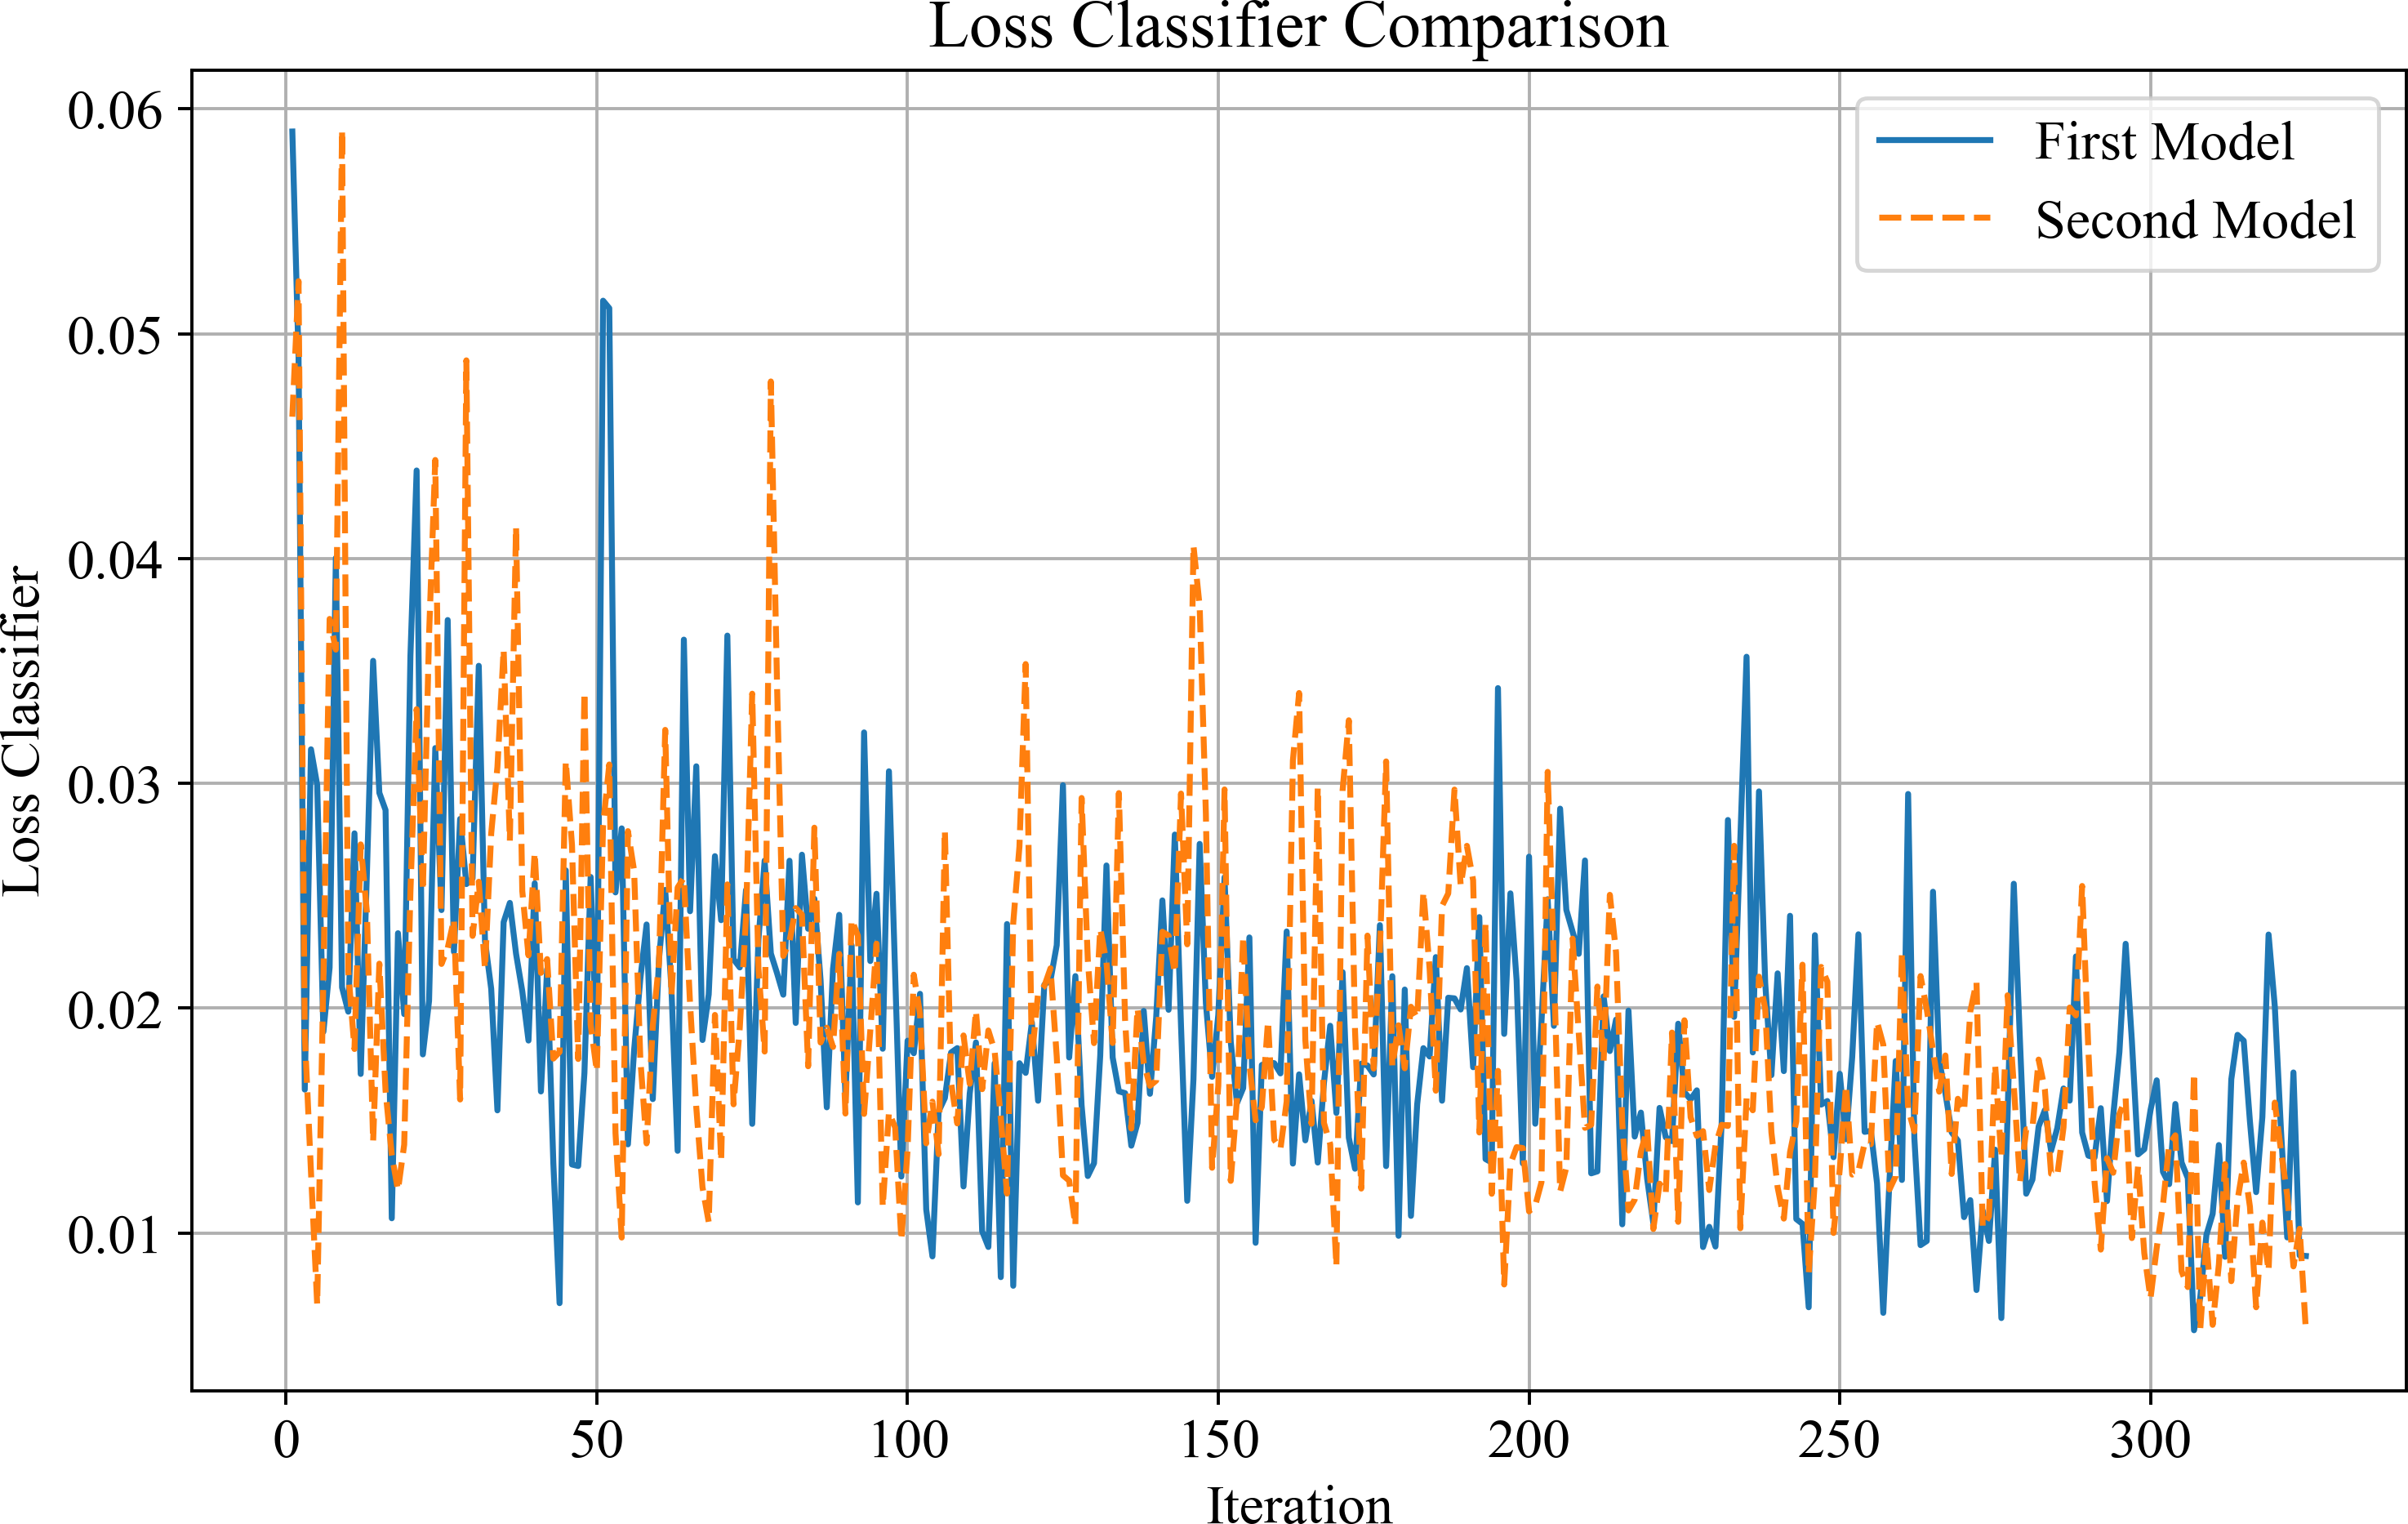
\includegraphics[width=0.8\textwidth]{media/ict/image23}
	\caption*{}
\end{figure}


{\bfseries 1-сурет. Екі модель үшін классификатор жоғалтуының графикалық
салыстырылуы}

\begin{figure}[H]
	\centering
	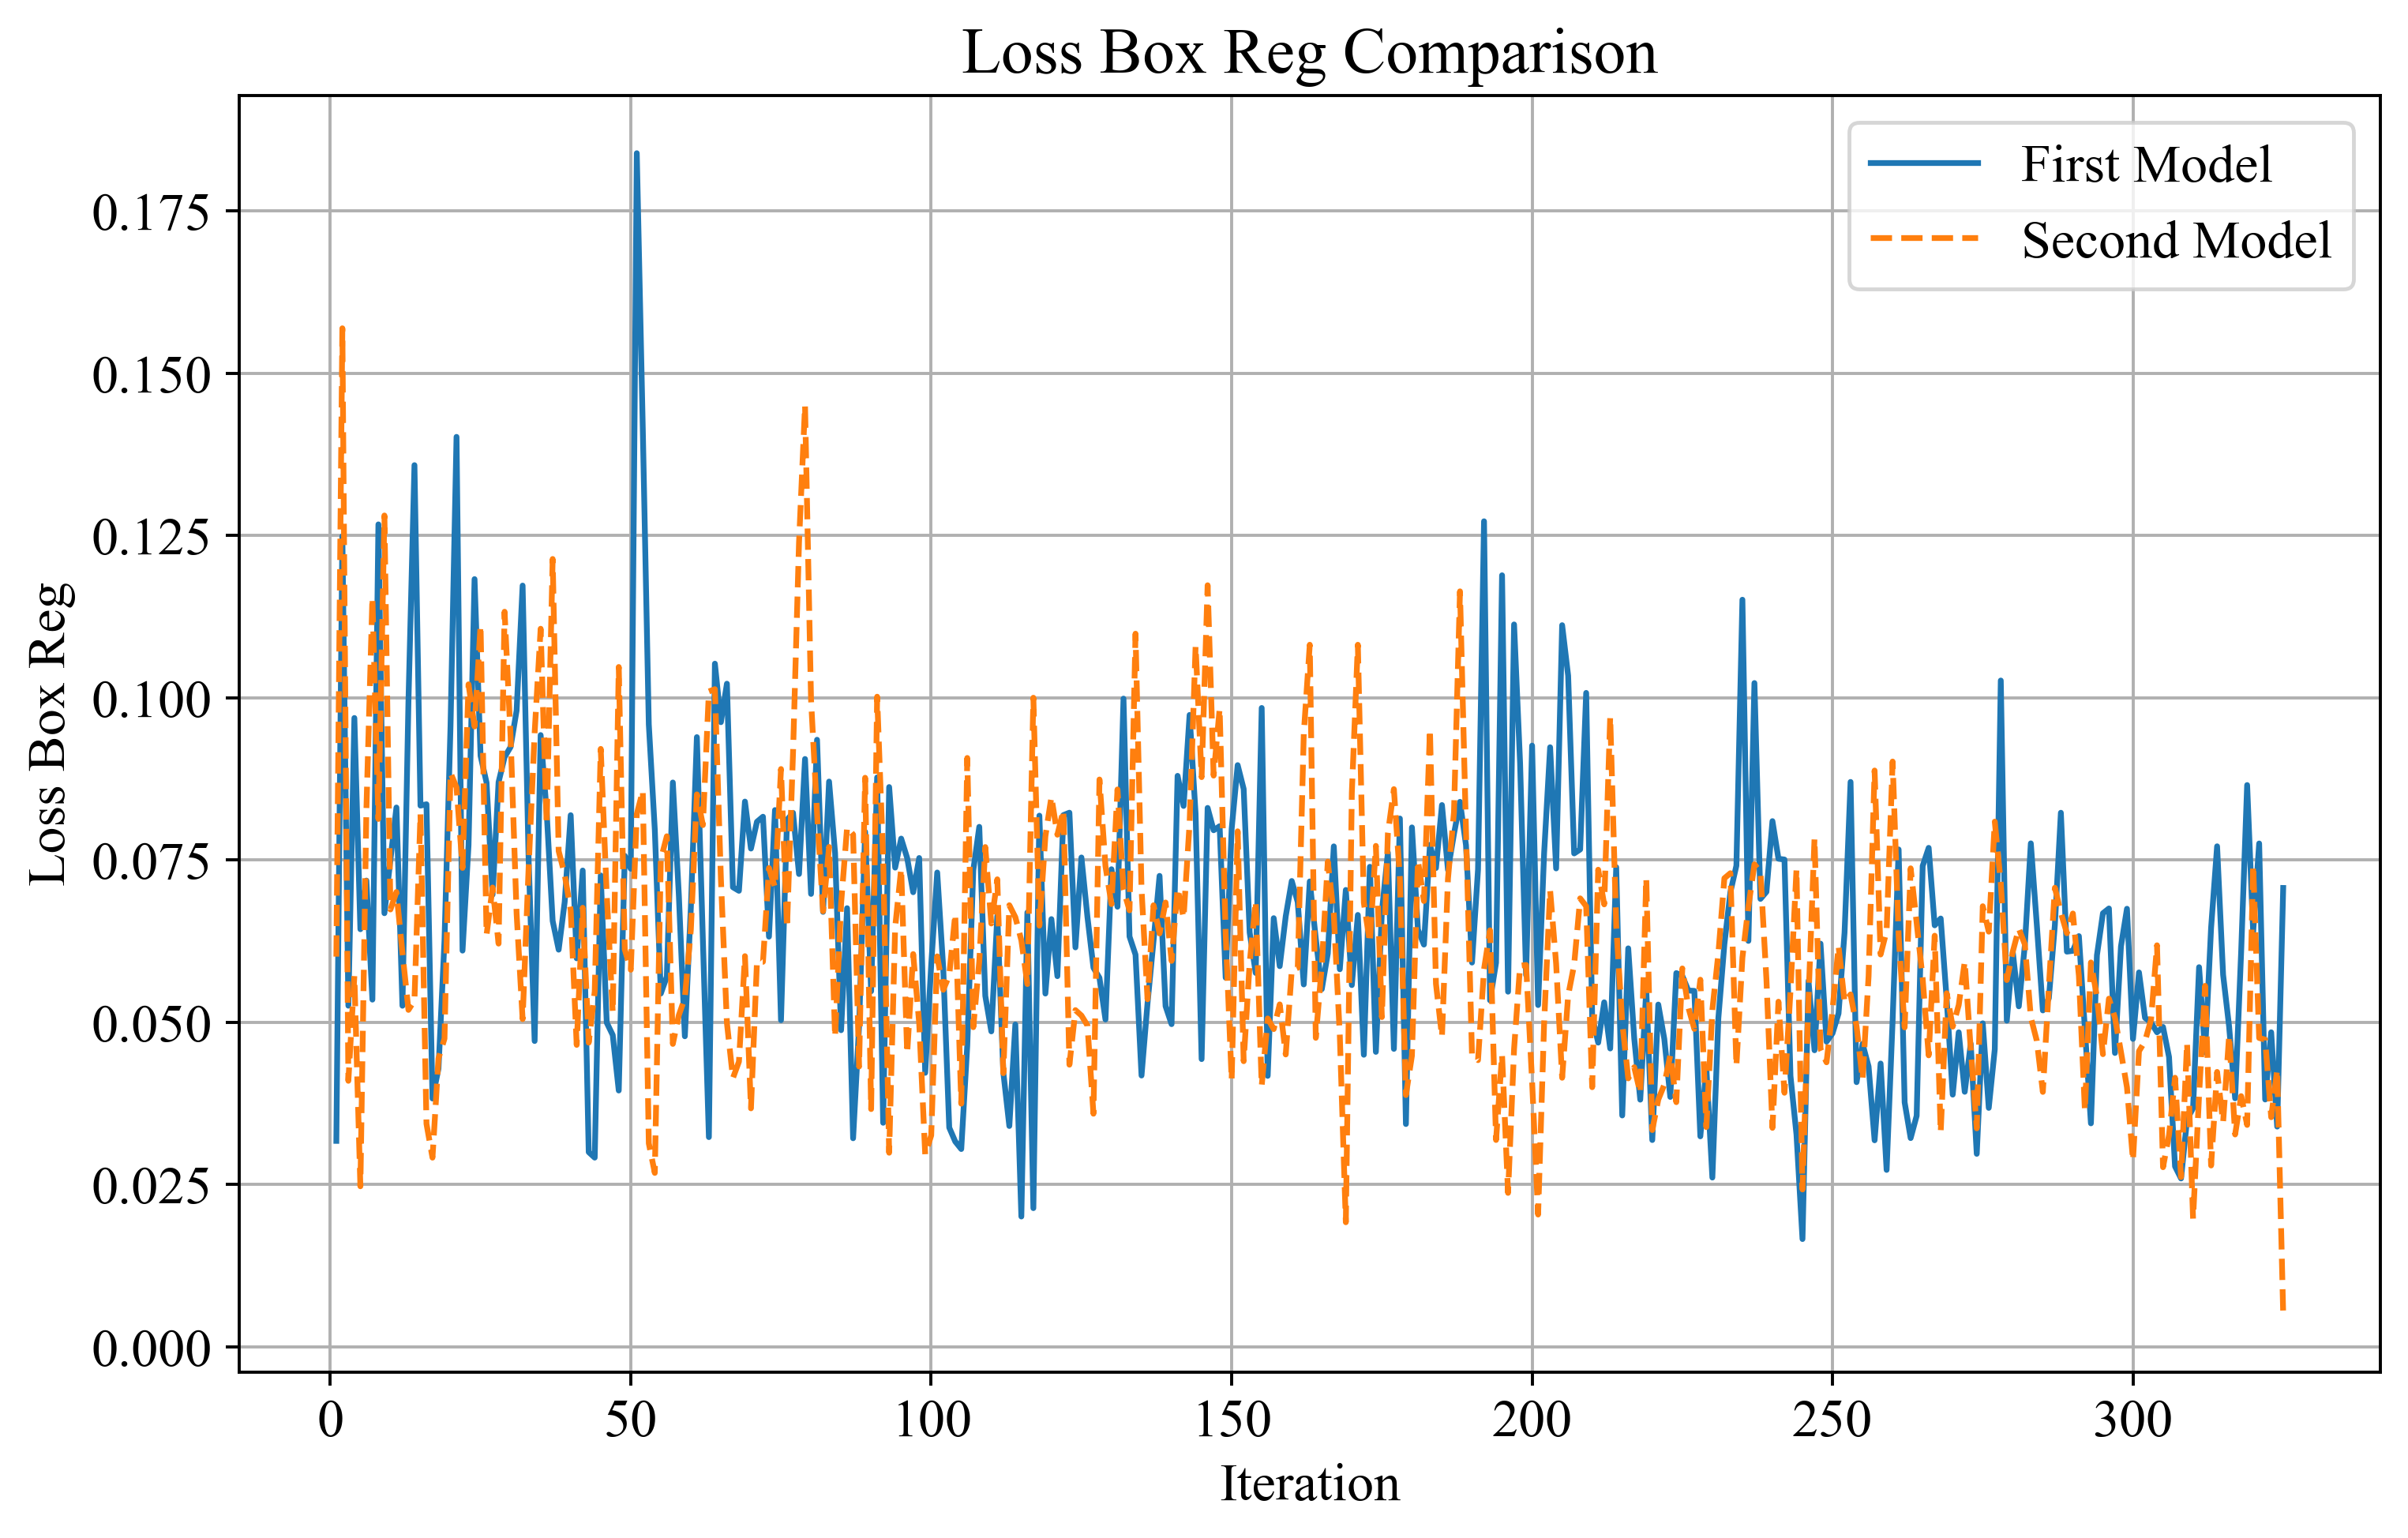
\includegraphics[width=0.8\textwidth]{media/ict/image24}
	\caption*{}
\end{figure}


{\bfseries 2-сурет. Екі модель арасындағы рамканың регрессия жоғалтуын
салыстыру}

Әдістеме Faster R-CNN-ның соңғы нәтижелеріне оқу моделінің мөлшері мен
түрлі оқу параметрлерінің әсерін талдауға бағытталған. Бұл сүт
бездерінің патологияларын анықтау кезінде максималды дәлдікке қол
жеткізу үшін оңтайлы параметрлер мен жағдайларды анықтауға мүмкіндік
береді. Соңғы нәтижелер мен қорытындылар медициналық тәжірибеде сүт безі
патологиясын жоғары дәлдікпен анықтаудың тиімді құралы ретінде Faster
R-CNN әдісін таңдаудың негізін құрайды. Әдістеме сонымен қатар, Faster
R-CNN арқылы анықталған патологияларды автоматтандырылған және қолмен
талдау механизмдерімен сапаны бақылау жүйесін құруды көздейді. Бұл кезең
нақты клиникалық тәжірибеде модель нәтижелерінің сенімділігі мен
дәлдігін тексеруге бағытталған. Анықталған өзгерістерді медициналық
мамандардың қолмен тексеруі патологияларды дәл анықтауға қосымша
сенімділік деңгейін қамтамасыз етеді, әсіресе жоғары дәлдік аса маңызды
болған жағдайда. Бұдан бөлек, әдістеме Faster R-CNN моделін нақты
уақытта немесе шын уақыт режимінде қолдану үшін қажетті есептеу
ресурстарын талдауды қамтиды. Бұл әзірленген әдісті диагностикалық
тиімділігі жоғары медициналық мекемелерге интеграциялау мүмкіндігін
қарастырған кезде маңызды аспект болып табылады. Faster R-CNN
нәтижелерін басқа машиналық оқыту әдістерімен және маммографиядағы
дәстүрлі тәсілдермен салыстыру сүт безі патологиясын анықтаудағы осы
әдістің артықшылықтарын айқындайды. Ұсынылған тәсіл диагностика сапасын
айтарлықтай жақсартуға және сүт безі ауруларын ерте анықтау арқылы
тиімділігін арттыруға мүмкіндік береді.

{\bfseries Нәтижелер және талқылау.} Бұл жұмыста біз сүт безі аномалияларын
анықтау үшін маммография деректер базасында оқытылған екі негізгі
модельді: Faster R-CNN және YOLOv8-ді қарастырамыз. Осы модельлердің
жаттығу нәтижелері жаттығу және валидацияның жоғалуы, дәлдік және
F1-өлшемі сияқты көрсеткіштер түрінде тіркелді. Faster R-CNN-ның оқыту
және валидация жоғалтуының графигі оқыту дәуірі барысында деректер
базасындағы жоғалтудың қалай төмендейтінін көрсетеді. Бұл модельдің
қателерді азайта отырып, жалпылау қабілетін сәтті жақсарып жатқанын
білдіреді. Қисықтардың конвергенциясы, сондай-ақ, оқу және валидация
деректер базасында жоғары дәлдік пен F1 көрсеткішінің байқалатындығы
артық сәйкестіктің жоқтығын көрсетеді. Faster R-CNN үшін оқыту және
тестілеу дәлдіктері әр дәуір сайын тұрақты түрде өсіп, жаттығудың
соңында шамамен 0,99 мәніне жетеді. Бұл модель деректердегі модельлерді
сәтті танып, болжамдарының барған сайын дәлірек болып келе жатқанын
көрсетеді. Осыған ұқсас жетістіктер 3-суретте көрсетілген F1 ұпайында
байқалады, ол дәлдік пен еске түсіру арасындағы тепе-теңдікті көрсетіп,
0,97-ге жақындайды.

\begin{figure}[H]
	\centering
	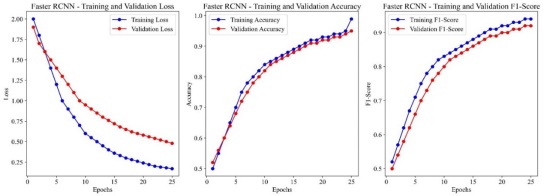
\includegraphics[width=0.8\textwidth]{media/ict/image25}
	\caption*{}
\end{figure}


{\bfseries 3-сурет. Faster R-CNN моделін оқыту нәтижелері}

Faster R-CNN сияқты, YOLOv8 де оқу процесінің табысты көрсеткіштерін
көрсетеді. Жаттығу және валидация деректеріндегі жоғалту графигі
бастапқы кезеңдерде жоғалтудың жылдам төмендеуін көрсетіп, модельдің
жоғары конвергенция жылдамдығын білдіреді. Жаттығу және валидация
деректер базасының дәлдігі мен F1-өлшемі, 4-суретте көрсетілгендей,
сәйкесінше шамамен 0,97 және 0,96 мәндеріне жетіп, дәйекті түрде
жақсарады. Екі модельні салыстыра отырып, олардың екеуі де жоғары
өнімділікті көрсететінін атап өту маңызды. Алайда, Faster R-CNN
YOLOv8-мен салыстырғанда, әсіресе оқудың соңғы кезеңдерінде дәлдік пен
F1-өлшеу мәндерінің аздап жоғары екенін айту керек. 5-суретте
көрсетілген модель патологияның әртүрлі деңгейлері бар 1318 кескінді
пайдалана отырып, сүт безі қатерлі ісігін жіктеуге арналған. Кескінді
өңдеу процесі патологиялық өзгерістерді анықтау үшін қалыпқа келтіру,
туралау және бүркемелеу қадамдарын қамтиды. YOLOv8 және Faster R-CNN
әдістерінің тиімділігін бағалау үшін патологияның әртүрлі формаларын
қамтитын 1318 кескіннен тұратын ауқымды деректер жинағы қолданылды.
Деректер жинағы қатерлі және қатерсіз кескіндер арасында теңгерілген
және сүт безі қатерлі ісігінің бес деңгейлі жіктелуін ұсынды. Бұл тәсіл
сүт безінің медициналық кескіндеріндегі патологияларды анықтау үшін екі
модельдің тиімділігін неғұрлым толық және объективті бағалауға мүмкіндік
береді.

\begin{figure}[H]
	\centering
	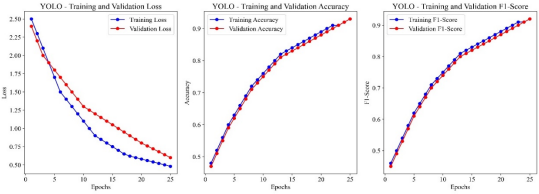
\includegraphics[width=0.8\textwidth]{media/ict/image26}
	\caption*{}
\end{figure}


{\bfseries 4-сурет. YOLOv8 модельсі бойынша оқыту нәтижелері}

\begin{figure}[H]
	\centering
	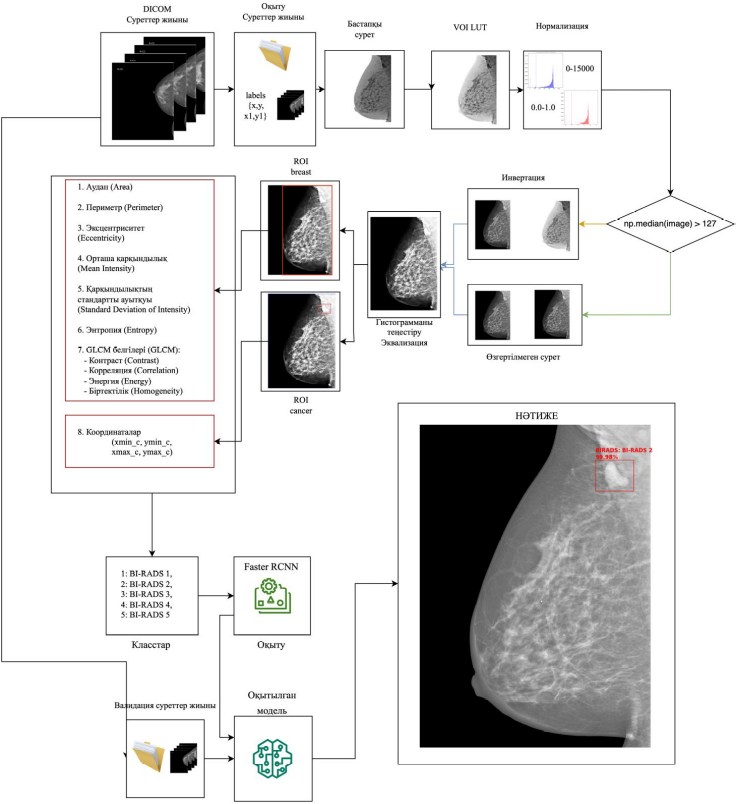
\includegraphics[width=0.8\textwidth]{media/ict/image27}
	\caption*{}
\end{figure}


{\bfseries 5-сурет. Сүт безі қатерлі ісігі патологиясын анықтау моделі}

Сүт безінің кескінін өңдеуге және жіктеуге арналған бұл әдіс тіндердің
денсаулығын жүйелі және жан-жақты бағалауды қамтамасыз етеді, бұл
медициналық қолданбалар үшін ерекше маңызды. Қалыпқа келтіру және
туралау әдістерін қолдану, сондай-ақ YOLOv8 және Faster R-CNN
алгоритмдерінің пайдаланылуы модельдің әртүрлі патологияларды анықтауда
жоғары сезімталдық пен дәлдікті көрсетуіне мүмкіндік береді. Әртүрлі
сыныптардан тұратын теңгерілген деректер базасы сүт безі патологиясының
әртүрлі формалары мен деңгейлерін ескере отырып, модельдің өнімділігін
неғұрлым өкілді бағалауға көмектеседі. Бұл тәсіл жіктеу нәтижелерінің
сенімділігін арттырады және сүт безі қатерлі ісігінің диагностикасын
айтарлықтай жақсартуға ықпал етеді.

{\bfseries Қорытынды.} Ұсынылған зерттеу маммографиялық кескіндердегі сүт
бездерінің патологиясын анықтау үшін YOLOv8 және Faster R-CNN терең
оқыту модельдерін тиімді пайдалану мүмкіндігін көрсетеді. Екі модель де
дәлдік, F1 ұпайы және өңдеу жылдамдығы бойынша жоғары нәтижелер
көрсетті, бұл олардың медициналық салада практикалық қолдану әлеуетін
айқындайды. Faster R-CNN моделі, әсіресе, жаттығудың соңғы кезеңдерінде
YOLOv8-ден дәлдік пен F1 ұпайы бойынша тұрақты түрде жоғары болды,
шамамен 0,99 дәлдік және 0,97 F1 ұпайына қол жеткізіп, сүт безі
ауытқуларын анықтаудағы сенімділігін көрсетті. YOLOv8, сәл төменірек
дәлдікке ие болғанымен, жоғары өңдеу жылдамдығын көрсетті, бұл оны
жылдам талдау талап етілетін қолданбалар үшін қолайлы етеді, ал оның
дәлдігі шамамен 0,97, F1 ұпайы 0,96 болды, бұл оның сүт безі
патологиясын анықтаудағы тиімділігін растайды. Деректерді алдын ала
өңдеу, оның ішінде қалыпқа келтіру, гистограмманы теңестіру және
аномалия аймақтарын маскалау, оқу процесінің тұрақтылығына және сүт
бездерінің патологияларын анықтауда модельлердің сенімділігіне елеулі
әсер етті. Екі модель де патологияның әртүрлі деңгейлерін қамтитын 1318
маммографиялық кескіннің теңгерілген деректер базасында оқытылды және
тексерілді, бұл олардың сүт безі ауруларының қатерсіз және қатерлі
формаларымен күресу қабілетін нығайтады. Бұл модельлерді клиникалық
тәжірибеге енгізу сүт безі ауруларын ерте анықтау мен диагностикалауды
жақсартуға, сондай-ақ пациенттердің нәтижелерін жақсартуға мүмкіндік
береді. Оқыту параметрлері мен модель архитектурасын оңтайландыруға,
деректер базасын кеңейтуге және модельдерді одан әрі жетілдіруге,
олардың шынайы клиникалық параметрлерде сенімділігі мен дәлдігін
қамтамасыз ету үшін қосымша зерттеулер жүргізу ұсынылады.

{\bfseries Әдебиеттер}

1. A. Orazayeva et al. Biomedical image segmentation method based on
contour preparation // in Photonics Applications in Astronomy,
Communications, Industry, and High Energy Physics Experiments. -- 2022.
DOI: 10.1117/12.2657929

2. Z. He, P. Wang, and X. Ye, Novel endoscopic optical diagnostic
technologies in medical trial research: recent advancements and future
prospects // BioMedical Engineering OnLine. -2021. -Vol. 20(1). DOI:
10.1186/s12938-020-00845-5

3. O. Yu. Bogaevskaya, A. V Yumashev, A. L. Zolkin, O. A. Smirnova, and
M. S. Chistyakov, Application of progressive information technologies in
medicine: computer diagnostics and 3D technologies // Journal of
Physics: Conference Series. -2021. - Vol. 1889(5). DOI:
10.1088/1742-6596/1889/5/052001

4. R. Boina et al. Enhancing intelligence diagnostic accuracy based on
machine learning disease classification // International Journal of
Intelligent Systems and Applications in Engineering. -2023. -Vol. 11.
-P. 765--774, 2023.

5. C.-H. Hsu et al. Effective multiple cancer disease diagnosis
frameworks for improved healthcare using machine learning //
Measurement. -2021. -Vol. 175. DOI: 10.1016/j.measurement.2021.109145

6. P. Singh, N. Singh, K. K. Singh, and A. Singh Diagnosing of disease
using machine learning // in Machine Learning and the Internet of
Medical Things in Healthcare. - Elsevier, 2021. - P. 89--111.

7. A. Orazayeva et al. Imaging fuzzy expert system for assessing dynamic
changes in biomedical tumor images in breast cancer // in Photonics
Applications in Astronomy, Communications, Industry, and High Energy
Physics Experiments 2022. -Dec. 2022. DOI: 10.1117/12.2657923.

8. A. Orynbayeva, N. Shyndaliyev, and A. Aripbayeva Improving
statistical methods of data processing in medical universities using
machine learning //World Transactions on Engineering and Technology
Education. -2023. -Vol. 21(1). -P. 58--63.

9. Y. Liu, D. Han, A. V Parwani, and Z. Li Applications of artificial
intelligence in breast pathology // Archives of Pathology \& Laboratory
Medicine. -2023. -Vol. 147(9). -P. 1003--1013. DOI:
10.5858/arpa.2022-0457-ra

10. Y. Li, Y. Zhang, Q. Yu, C. He, and X. Yuan Intelligent scoring
system based on dynamic optical breast imaging for early detection of
breast cancer // Biomedical Optics Express. -2024. -Vol. 15(3). -P.
1515--1527. DOI: 10.1364/BOE.515135

11. E. A. Rakha, G. M. Tse, and C. M. Quinn An update on the
pathological classification of breast cancer // Histopathology. -2022.
-Vol. 82(1). -P. 5--16. DOI: 10.1111/his.14786

12. C. Quinn, A. Maguire, and E. Rakha Pitfalls in breast pathology //
Histopathology. -Vol. 82(1). -P. 140--161. DOI: 10.1111/his.14799

13. M. Ensenyat-Mendez et al. Current triple-negative breast cancer
subtypes: dissecting the most aggressive form of breast cancer //
Frontiers in Oncology. -2021. -Vol. 11. DOI: 10.3389/fonc.2021.681476

14. S. Iranmakani et al. A review of various modalities in breast
imaging: technical aspects and clinical outcomes // Egyptian Journal of
Radiology and Nuclear Medicine. -2020. -Vol. 51(1). DOI:
10.1186/s43055-020-00175-5

15. S. M. H. Hashemi, L. Safari, and A. D. Taromi Realism in action:
anomaly-aware diagnosis of brain tumors from medical images using YOLOv8
and DeiT. -2024. DOI: 10.48550/arXiv.2401.03302

16. R.-Y. Ju and W. Cai Fracture detection in pediatric wrist trauma
X-ray images using YOLOv8 algorithm // Scientific Reports. -2023.-Vol.
13(1). DOI: 10.1038/s41598-023-47460-7

17. S. Pandey, K.-F. Chen, and E. B. Dam Comprehensive multimodal
segmentation in medical imaging: combining YOLOv8 with SAM and HQ-SAM
models // 2023 IEEE/CVF International Conference on Computer Vision
Workshops (ICCVW). - Paris, France, 2023. -P. 2584-2590. DOI:
10.1109/iccvw60793.2023.00273

18. B. W. Choi, S. Kang, H. W. Kim, O. D. Kwon, H. D. Vu, and S. W. Youn
Faster region-based convolutional neural network in the classification
of different parkinsonism patterns of the striatum on maximum intensity
projection images of {[}18F{]} FP-CIT positron emission tomography //
Diagnostics. -2021. -Vol. 11(9). DOI: 10.3390/diagnostics11091557

19. Z. Jiao et al. Deep learning for automatic detection of
cephalometric landmarks on lateral cephalometric radiographs using the
Mask Region-based Convolutional Neural Network: a pilot study // Oral
Surgery, Oral Medicine, Oral Pathology and Oral Radiology. -2024. -Vol.
137(5). -P. 554--562. DOI: 10.1016/j.oooo.2024.02.003

20. A. Orazayeva, J. Tussupov, W. Wójcik, S. Pavlov, G. Abdikerimova,
and L. Savytska Methods for detecting and selecting areas on texture
biomedical images of breast cancer // Informatyka, Automatyka, Pomiary w
Gospodarce i Ochronie Srodowiska. -2022. -Vol. 12(2). -P. 69--72. DOI:
10.35784/iapgos.2951

21. G. Abdikerimova et al. Detection of lung pathology using the fractal
method // International Journal of Electrical and Computer Engineering.
-2023. -Vol. 13(6). -P. 6778--6786. DOI:
10.11591/ijece.v13i6.pp6778-6786

22. G. Abdikerimova et al. Detection of chest pathologies using
autocorrelation functions // International Journal of Electrical and
Computer Engineering. -2023. -Vol. 13(4). -P. 4526--4534. DOI:
10.11591/ijece.v13i4.pp4526-4534

23. Zaridze D.G., Maksimovich D.M. Prevention of malignant neoplasms. //
V-Petersburg International Oncology Forum. Collection. - 2017. - No. 4
(2). DOI: 10.17650/2313805X-2017-4-2-8-25

24. Davydov M.I., Zaridze D.G. Skrining zlokachestvennyh opuholej //
Vestnik FGBNU «RONC im N.N. Blohina». -2014. --T. 25. -№3-4. --S. 5-16.
URL:https://cyberleninka.ru/article/n/skrining-zlokachestvennyh-opuholey/viewer
{[}in Russian{]}

25. Nurmanova A., Sultanova Z.I., Y.A. Annaorazov Y.A. Faktory i ih
rol'{} v zabolevaemosti, smertnosti, vyzhivaemosti pri
rake molochnoj zhelezy // Vestnik KazNMU. -2018. -№ 1. URL:
\url{https://cyberleninka.ru/article/n/faktory-i-ih-rol-v-zabolevaemosti-smertnosti-vyzhivaemosti-pri-rake-molochnoy-zhelezy/viewer}
{[}in Russian{]}

26. Chen L. et al. Review of image classification algorithms based on
convolutional neural networks //Remote Sensing. -- 2021. --Vol.13(22).
DOI:10.3390/rs13224712

27. N. Diniz D. et al. A deep learning ensemble method to assist
cytopathologists in pap test image classification //Journal of Imaging.
-2021. -Vol. 7(7). DOI:10.3390/jimaging7070111

{\bfseries Авторлар туралы мәліметтер}

Тусупов Д.А. -- физика-математика ғылымдарының докторы, профессор, Л.Н.
Гумилев атындағы Еуразия ұлттық университеті, Астана, Қазақстан, e-mail:
\href{mailto:oaris.83@gmail.com}{tussupov@mail.ru};

Оразаева А.Р. - Л.Н. Гумилев атындағы Еуразия ұлттық университетінің
докторанты, Ақпараттық жүйелер мамандығы, Астана, Қазақстан, e-mail:
oar\_is@mail.ru.

{\bfseries Information about the authors}

Tussupov J.A. - doctor of physical and mathematical sciences, professor,
L.N. Gumilev Eurasian National University, Astana, Kazakhstan, e-mail:
tussupov@mail.ru;

Orazayeva A.R. - L.N. Ph.D. student of Gumilev Eurasian National
University, Information Systems specialty, Astana, Kazakhstan, e-mail:
oar\_is@mail.ru.
